%%% fs-seim-optimistic - Optimistic approach

\label {fs-optimistic}

The main idea of our method is to represent stateful transformations as a sequence of a map and a windowed grouping operations and handle out-of-order items within them. 

Following our approach, we make some assumptions about stream processing system, that is suitable for applying it. Such system must support meta-information on data items, allow cycles in the logical graph, and its set of predefined operations must be sufficient to express map and windowed grouping operations.

In this section, firstly, we define the ordering model of data items. Then, we show that any stateful transformation can be implemented using the combination of windowed grouping and map operations. After that, we demonstrate an optimistic approach to handle out-of-order items within these operations. In the end of the section, the limitations of such technique are discussed.

\subsection{Ordering model}
We assume that there is a total order on meta-information of data items. Besides, ordering is preserved, when an item is going through the operations. More precisely, the order of output items is the same as the order of corresponding input items. Moreover, the output follows corresponding input but precedes the next item. The ordering model is shown in the figure ~\ref{ordering}.

\begin{figure}[htbp]
  \centering
  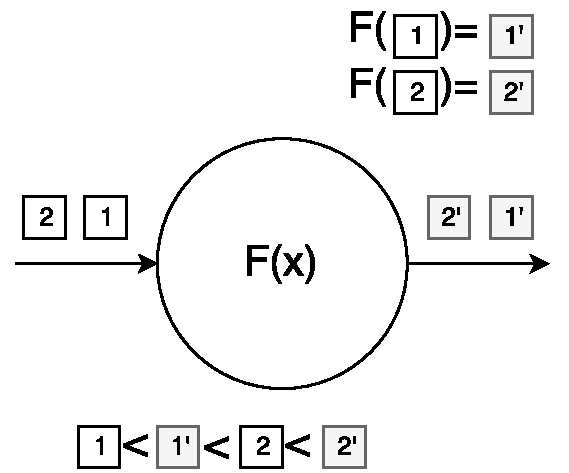
\includegraphics[width=0.48\textwidth]{pics/ordering}
  \caption{Ordering}
  \label {ordering}
\end{figure}

\subsection{Semantics of map and windowed grouping operations}

\subsubsection{Map}
Map transforms input item into a sequence of its derivatives, according to a function on item's payload provided by a user. This sequence can consist of any number of items or even be empty.

\subsubsection{Windowed grouping}
Windowed grouping is a stateful operation with a numeric parameter {\it window}. It is supposed that payloads of input items of grouping operation have key-value form. The state of this operation is represented by a set of buckets, one for each key. Windowed grouping has the following semantics:

\begin{itemize}
    \item Each input item is put into the corresponding bucket at position defined by its meta-information
    \item The output of grouping operation is a window-sized tuple of the last items in the corresponding bucket. If bucket size is less than window, the output contains full bucket
\end{itemize}

The following example illustrates the semantics of the windowed grouping operation. In this example, payloads of input items are represented as natural numbers: 1, 2, 3, etc. The hash function returns 1 if the number is even and 0 otherwise. If the window is set to 3, the output is:

\[(1), (2), (1|3), (2|4), (1|3|5), (2|4|6), (3|5|7), (4|6|8)...\]

\subsection{Stateful transformations using defined operations}
Figure ~\ref{stateful-schema} shows the part of the logical pipeline, that can be used for stateful transformation. The input of windowed grouping operation is supposed to be ordered. There are several functional steps to produce output and update state. These steps can be detailed by considering two cases:

\begin{itemize}
    \item When the first item arrives at grouping, it is inserted into the empty bucket. Grouping outputs single-element tuple, and then it is sent to the combined map. Combined map generates state object and sends it back to the grouping in the form of an ordinal key-value data item. The key of the state item is the same as in the item in tuple and value is the state. Combined map can generate some additional output and send it further down the stream
    \item When new regular input item arrives at windowed grouping, it is inserted into the corresponding bucket's tail, because of the order assumptions. Additionally, the right ordering guarantees that input item is grouped into the tuple with previously generated state item. The next map operation combines new item and previous state into the new state item. After that, the new state item is returned to the grouping through the cycle. As in the preceding case, combined map can generate some additional output
\end{itemize}

\begin{figure}[htbp]
  \centering
  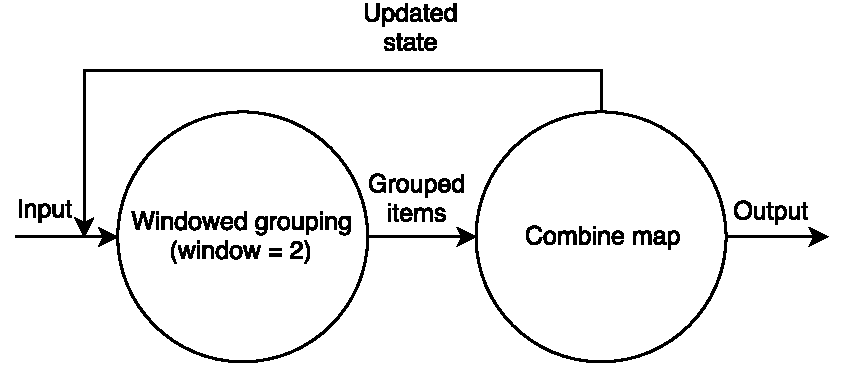
\includegraphics[width=0.48\textwidth]{pics/stateful-schema}
  \caption{The part of the logical pipeline for stateful transformation}
  \label {stateful-schema}
\end{figure}

The example of square matrix multiplication within proposed approach is shown in the figure ~\ref{matrix-example}. In this example, input items are represented as key-value pairs, where the key is the dimension of a matrix and the value is the matrix itself. The reaction on three input matrices are the following:

\begin{itemize}
    \item When the first matrix {\it A} arrives at grouping, it is put into the empty bucket for 3x3 matrices. After that, the single-element tuple with matrix {\it A} is sent to combine map operation. Combine map creates state object for matrix {\it A}, which is actually just {\it A} itself. In the last step, state item is sent back to grouping, and it is inserted right after item for matrix {\it A}
    \item Matrix {\it B} is arrived and inserted into the bucket right after state item. The tuple containing state item and item for matrix {\it B} is sent to combine map. Combine map multiplies matrix in the state by matrix {\it B}. The result of this operation is matrix {\it AB}. New state item for matrix {\it AB} is created and sent back to the grouping. It is inserted in bucket right after item with matrix {\it B}
    \item Matrix {\it C} is arrived and went through the pipeline in a similar way as matrix {\it B}
\end{itemize}

\begin{figure}[htbp]
  \centering
  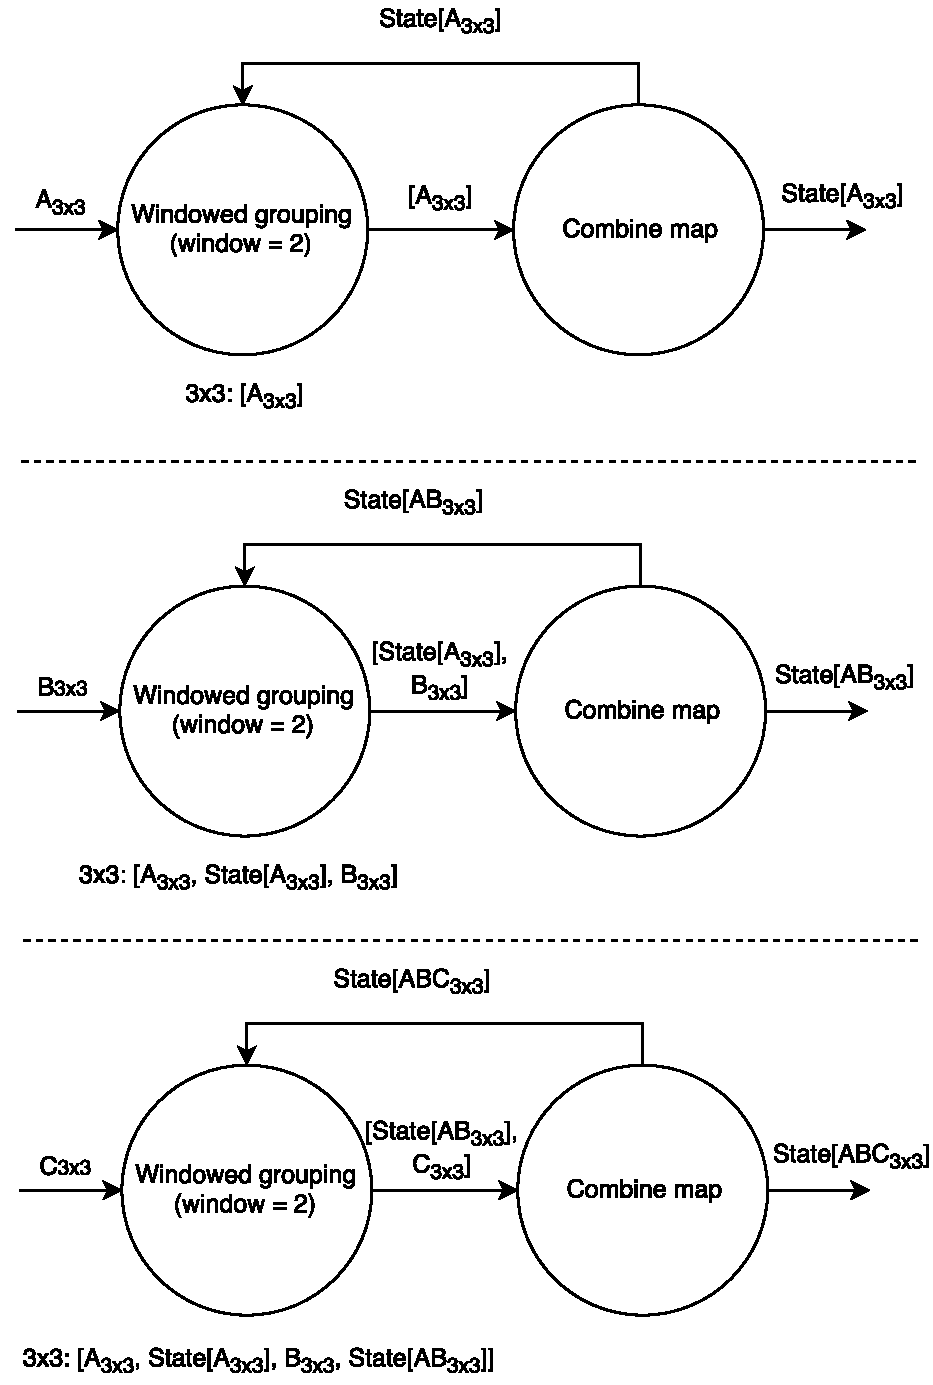
\includegraphics[width=0.48\textwidth]{pics/matrix-example}
  \caption{Matrix multiplication example}
  \label {matrix-example}
\end{figure}

\subsection{Handling out-of-order events}

\subsection{Limitations}




